\section{Обратное проектирование вознаграждения}

\subsection{Ключевые идеи}

В статье~\cite{hadfieldmenell2020inverse} рассматривается функция вознаграждения как наблюдение, сделанное в контексте конкретной среды, и позволяет вывести распределение возможных истинных целей.  
Это помогает избежать негативных последствий ошибочной спецификации вознаграждения, таких как побочные эффекты или манипулирование системой вознаграждения.

В основе метода лежит идея о том, что функция вознаграждения, заданная человеком, не является точным выражением его намерений, а лишь приближённым отражением желаемого поведения агента. Анализируя контекст, в котором эта функция была создана, можно восстановить вероятностное распределение истинных целей и оценить, какие функции вознаграждения могли бы привести к схожему поведению в обучающей среде. Агент, обладающий таким распределением, способен учитывать неопределённость в своих оценках и принимать решения, минимизирующие риск попадания в нежелательные состояния или совершения опасных действий.

\subsection{Математическое описание метода}

Предполагается, что проектировщик выбирает приближённую функцию вознаграждения $\tilde{w}$  так, чтобы максимизировать ожидаемое истинное вознаграждение.  
Тогда вероятность выбора этой функции описывается выражением:
\begin{equation}
P(\tilde{w} \mid w^{*}, \tilde{M}) \propto 
\exp\left(
\beta \, \mathbb{E}_{\xi \sim \pi(\xi \mid \tilde{w}, \tilde{M})}
[w^{*\top} \phi(\xi)]
\right),
\end{equation}
где $w^{*}$~-- истинные веса вознаграждения, $\phi(\xi)$~-- вектор признаков траектории, $\pi(\xi \mid \tilde{w}, \tilde{M})$~-- распределение траекторий, а $\beta$~-- степень рациональности проектировщика.

Апостериорное распределение для истинной функции вознаграждения вычисляется как:
\begin{equation}
P(w^{*} \mid \tilde{w}, \tilde{M}) \propto
\frac{
\exp(\beta w^{\top} \tilde{\phi})
}{
\tilde{Z}(w)
} P(w),
\end{equation}
где нормализующая константа:
\begin{equation}
\tilde{Z}(w) = \int_{\tilde{w}} \exp(\beta w^{\top} \tilde{\phi}) \, d\tilde{w}.
\end{equation}

\subsection{Алгоритм}

Алгоритм обратного проектирования вознаграждения включает последовательность шагов:

\begin{enumerate}
    \item \emph{Решение тренировочного мира.}  
    Агент обучается в тренировочной среде $\tilde{M}$ с функцией вознаграждения $\tilde{w}$, вычисляя ожидаемые признаки траекторий $\tilde{\phi}$.  
    На этом этапе он действует в среде без лавы, как показано на левой панели рисунка~\ref{fig:lavaland_behavior}.
    
    \item \emph{Построение апостериорного распределения.}  
    На основе наблюдаемой прокси-функции вычисляется распределение вероятностей для возможных истинных функций вознаграждения $P(w^{*} \mid \tilde{w}, \tilde{M})$.  
    Это распределение отражает неопределённость относительно предпочтений проектировщика.
    
    \item \emph{Оценка риска.}  
    Агент анализирует дисперсию вознаграждения для разных состояний среды. В тестовой среде, содержащей лаву (см. центральную панель рисунка~\ref{fig:lavaland_behavior}), высокая неопределённость указывает на потенциальную опасность.
    
    
    \item \emph{Планирование с учётом риска.}  
    Используется стратегия риск-избегающее планирование: агент минимизирует ожидаемые потери от ошибочной интерпретации цели, избегая состояний с высокой неопределённостью.  
    В результате он прокладывает безопасный маршрут (правая панель рисунка~\ref{fig:lavaland_behavior}), выбирая траекторию, согласованную с вероятностной моделью среды.
\end{enumerate}

\begin{figure}[h!]
    \centering
    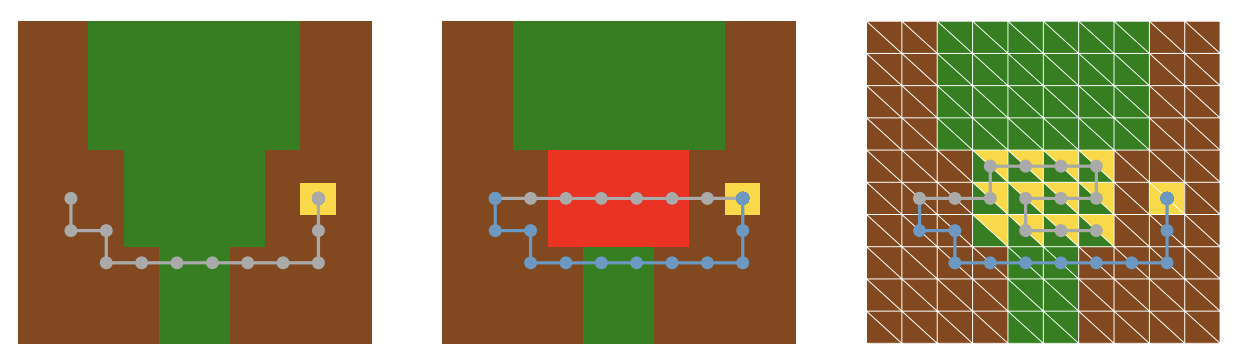
\includegraphics[width=0.9\linewidth]{images/Аgent_behavior_in_Lavaland_env.png}
    \caption{Примеры поведения агента. Слева~-- тренировочная среда без лавы, посередине~-- тестовая с лавой, справа~-- тестовая среда с некоррелирующими сенсорами. Серый путь~-- поведение при буквальном следовании прокси-функции, синий~-- поведение после применения обратного проектирования вознаграждения.}
    \label{fig:lavaland_behavior}
\end{figure}

\subsection{Наборы данных}

Для экспериментов используется искусственный мир \emph{Лавалэнд (Lavaland)}~-- двумерная сетка, содержащая четыре типа местности: цель, трава, грунт и лава.  
Истинная функция вознаграждения поощряет быстрое достижение цели и избегание лавы и травы.  
Тренировочная среда не содержит лавы, а тестовая добавляет этот тип местности.  
Общая структура среды и распределение признаков для каждого типа местности представлены на рисунке~\ref{fig:lavaland_latent_model}.


\begin{figure}[h!]
    \centering
    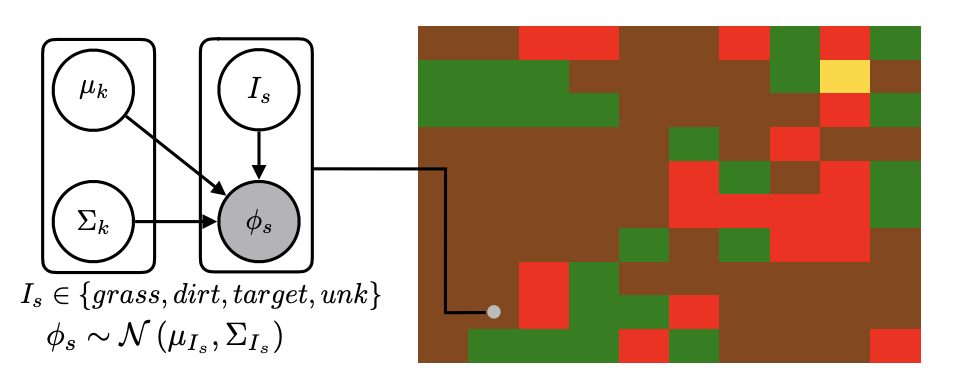
\includegraphics[width=0.8\linewidth]{images/Latent_model_of_Lavaland_env_feats.png}
    \caption{Модель среды Лавалэнд. Каждому типу местности (трава, грунт, цель, лава) соответствует распределение признаков $\phi_{s} \sim \mathcal{N}(\mu_{I_{s}}, \Sigma_{I_{s}})$. Агент должен избегать лавы, даже если она не имеет явного индикатора.}
    \label{fig:lavaland_latent_model}
\end{figure}

Рассматриваются два типа задач:
\begin{itemize}
    \item демонстрационные примеры с явными признаками всех типов местности;
    \item задачи с \emph{латентными признаками}, где каждый тип местности соответствует нормальному распределению признаков:
    \begin{equation}
    \phi_{s} \sim \mathcal{N}(\mu_{I_{s}}, \Sigma_{I_{s}}), \quad I_{s} \in \{\text{трава}, \text{грунт}, \text{цель}, \text{лава}\}.
    \end{equation}
\end{itemize}

\subsection{Метрики}

Для оценки эффективности алгоритма используются следующие метрики:
\begin{itemize}
    \item \emph{Доля столкновений с лавой}~-- основная метрика, показывающая, насколько часто агент попадает в клетки с лавой при планировании маршрута в тестовой среде.
    \item \emph{Средняя длина траектории}~-- позволяет оценить, насколько избегание лавы влияет на эффективность достижения цели.
    \item \emph{Разница между ожидаемым и истинным вознаграждением}~-- характеризует степень несоответствия между намерениями проектировщика и фактическим поведением агента.
    \item \emph{Оценка риска по состояниям}~-- вычисляется на основе дисперсии апостериорного распределения $P(w^{*} \mid \tilde{w}, \tilde{M})$ и отражает уверенность агента в своих решениях.
\end{itemize}

\subsection{Результаты}

Метод обратного проектирования вознаграждения снижает вероятность попадания агента в опасные зоны и предотвращает манипулирование функцией вознаграждения. Он обеспечивает устойчивое поведение даже при отсутствии явных признаков опасных состояний.  

На рисунке~\ref{fig:results} показано, что оба варианта аппроксимации (\emph{MaxEnt Z} и \emph{Sample Z}) значительно уменьшают долю траекторий, проходящих через лаву, по сравнению с агентом, использующим прокси-функцию напрямую.

\begin{figure}[h!]
    \centering
    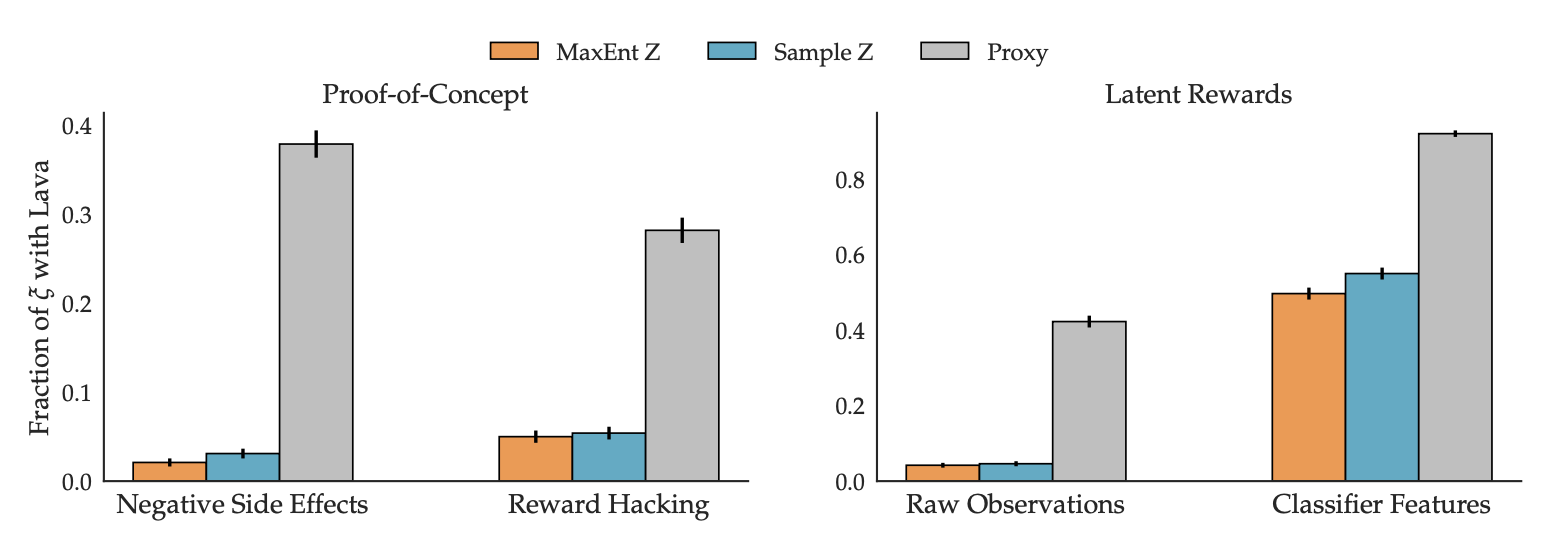
\includegraphics[width=0.85\linewidth]{images/IRD_results_comparison.png}
    \caption{Результаты экспериментов. Сравнение доли траекторий, проходящих через лаву, для базового метода (Proxy) и двух вариантов аппроксимации: \emph{MaxEnt Z} и \emph{Sample Z}.}
    \label{fig:results}
\end{figure}


